\chapter{Computer Vision}

% ---------- Pixel Accuracy ----------
\clearpage
\thispagestyle{cvstyle}
\section{Pixel Accuracy}
\subsection{Pixel Accuracy}

Pixel Accuracy is one of the most straightforward evaluation metrics for image segmentation tasks. It measures the proportion
of correctly classified pixels across the entire image, comparing the predicted segmentation mask to the ground truth.

\begin{center}
    FORMULA GOES HERE
\end{center}

A Pixel Accuracy of 1.0 indicates perfect segmentation, while lower values suggest a higher proportion of misclassified pixels.
A common variation, Mean Pixel Accuracy (MPA), calculates accuracy per class and then averages across all classes.
This adjustment ensures that smaller classes are not overshadowed by dominant ones, making MPA a more balanced evaluation
metric in class-imbalanced datasets.

\textbf{When to use Pixel Accuracy?}

Pixel Accuracy is useful when evaluating segmentation models where all pixel classes are of similar importance.
It provides a simple and interpretable measure of segmentation performance, making it a good starting point for initial
evaluation.

\coloredboxes{
\item Simple and interpretable.
\item Provides an initial sense of segmentation quality.
}
{
\item Insensitive to class imbalance. Heavily biased towards majority classes, leading to overly optimistic
evaluations in datasets with dominant background pixels.
\item Cannot differentiate per-class performance. A high Pixel Accuracy does not guarantee that all classes are well-segmented.
}

% ---------- PCK ----------
\clearpage
\thispagestyle{cvstyle}
\section{PCK}
\subsection{Percentage of Correct Keypoints}

Percentage of Correct Keypoints (PCK) is a popular metric in computer vision, specifically for evaluating human pose estimation
and keypoint detection models. It measures the percentage of detected keypoints that fall within a certain distance threshold
from the ground truth keypoints.

\begin{center}
    FORMULA GOES HERE
    % $PCK = \frac{Number of correctly predicted keypoints}{Total keypoints}$
\end{center}

A prediction is considered correct if the Euclidean distance between the predicted keypoint $K_p$ and the ground truth
keypoint $K_g$ is within a predefined threshold $\tau \geq ||K_p - K_g||$. The threshold $\tau$ is often defined
relative to an object or body part size, such as $PCK@0.2$ (20\% of the torso length) or $PCKh@0.5$ (50\% of the head size).

\textbf{When to use PCK?}

PCK is commonly used in tasks requiring keypoint localization, such as human pose estimation, object keypoint detection,
and facial landmark detection. It is particularly useful when the absolute pixel error is not meaningful due to variations
in object size.

\coloredboxes{
\item Scale Invariance. By normalizing the threshold based on body part size or image scale, PCK accounts for different
object sizes.
\item Robust to minor localization errors. Small deviations from the exact keypoint location do not significantly impact
the score.
}
{
\item The performance can vary significantly depending on the chosen threshold $\tau$, making comparisons difficult across
studies.
\item Not Differentiable. Since it is a threshold-based metric, it cannot be directly used as a loss function for training
deep learning models.
}

% ---------- OKS ----------
\clearpage
\thispagestyle{cvstyle}
\section{OKS}
\subsection{Object Keypoint Similarity}

Object Keypoint Similarity (OKS) is a key metric for evaluating keypoint-based object detection models, especially in human
pose estimation tasks. It is designed to measure how closely predicted keypoints match the ground truth, considering factors
like object scale and keypoint visibility.

\begin{center}
    FORMULA GOES HERE
\end{center}

OKS is analogous to Intersection over Union (IoU) for bounding boxes but applied to keypoint detection, providing a continuous
similarity score rather than a strict pass/fail threshold. It ranges from 0 to 1, where 1 indicates a perfect match.

\textbf{When to use OKS?}

OKS is particularly suited for evaluating pose estimation and keypoint-based object detection models, such as: human pose
estimation, facial landmark detection and benchmarking keypoint models.


\coloredboxes{
\item Scale-invariant evaluation. Unlike raw pixel-based metrics, OKS normalizes errors relative to object size,
ensuring fair evaluation across small and large objects.
\item Smooth penalization of localization errors.
Instead of a hard threshold (like in PCK), OKS applies a Gaussian function to penalize errors, making it a more continuous
and informative measure.
\item Handles occlusions and visibility issues. The visibility flag $v_i$ ensures that models are not penalized for missing
occluded or unlabeled keypoints.
}
{
\item Requires keypoint-specific constants. The $k_i$ values must be tuned per dataset, making cross-dataset comparisons
challenging.
\item Computationally more complex than PCK.
}

\clearpage
\orangebox{Did you know that...}
{OKS is the standard metric for evaluating pose estimation models in the COCO Keypoint Challenge, influencing the development
of state-of-the-art architectures like OpenPose, HRNet, and DEKR.}


% ---------- PSNR ----------
\clearpage
\thispagestyle{cvstyle}
\section{PSNR}
\subsection{Peak Signal-to-Noise Ratio}

In image generation and reconstruction, it is important to measure how closely the generated images resemble reference images.
PSNR is a widely used metric that quantifies pixel-level differences.

% equation
\begin{center}
    \tikz{
        \node[inner sep=2pt, font=\Large] (a) {
            {
                $\displaystyle
                    PSNR = 10 \cdot \log_{10}\left(\frac{\color{nmlred}MAX^2}{\color{nmlpurple}MSE}\right)
                $
            }
        };
        \draw[-latex,nmlred, semithick] ($(a.north)+(2.1,-0)$) to[bend right=15] node[pos=1, left] {maximum possible pixel}
        +(-1,.5); 
        \draw[-latex,nmlpurple, semithick] ($(a.south)+(2,-0.1)$) to[bend left=15] node[pos=1, left] {mean squared error}
        +(-1,-.5);
    }
\end{center}

\vspace{-10pt} 

where given an original image $O$ of size $h \times w$ and a reconstructed image $R$, the $MSE$ is defined as:

\vspace{-10pt}

% equation
\begin{center}
    \tikz{
        \node[inner sep=2pt, font=\large] (a) {
            {
                $\displaystyle
                 MSE = \frac{1}{\color{teal!70!green}h \cdot \color{nmlcyan}w} \sum_{i=1}^{h} \sum_{j=1}^{w}
                 \left(\color{nmlred} O(i,j) \color{black} - \color{nmlpurple} R(i,j) \right)^2
                $
            }
        };
        \draw[-latex,teal!70!green, semithick] ($(a.west)+(1.7,-0.5)$) to[bend left=15] node[pos=1, left] {height} +(-1,-.5); 
        \draw[-latex,nmlcyan, semithick] ($(a.west)+(2.4,-0.5)$) to[bend right=15] node[pos=1.62, left] {width} +(1,-.5);
        \draw[-latex,nmlred, semithick] ($(a.south)+(1,0.5)$) to[bend right=15] node[pos=1, right] {original pixel value}
        +(1,-.5);
        \draw[-latex,nmlpurple, semithick] ($(a.north)+(2.3,-0.4)$) to[bend right=15] node[pos=1, left] {reconstructed pixel
        value} +(-1,.5);    
    }
\end{center}

\vspace{-10pt}

The intuition behind PSNR is that it expresses how large the possible signal value is in comparison to the error. 
If the error is subtle compared to the maximum signal (i.e., a high PSNR), the reconstructed image is relatively similar to
the target in terms of pixel values. The unit of peak signal-to-noise ratio is decibel (dB) and the image have PSNR from 30 dB
could be consider as good reconstruction quality.



\textbf{When to use PSNR?}

PSNR is often chosen as the first metric to provide an overview of how closely the generated image matches the target.

\coloredboxes{
\item It is a straightforward and widely accepted standard for comparing vision algorithms.
\item Simple and fast to compute.
}
{
\item It is not always align with human perception of image.
\item PSNR is sensitive to even small global changes in lighting, contrast, or color.
}

\clearpage

\thispagestyle{customstyle}


\begin{figure*}[ht!]
    \centering
    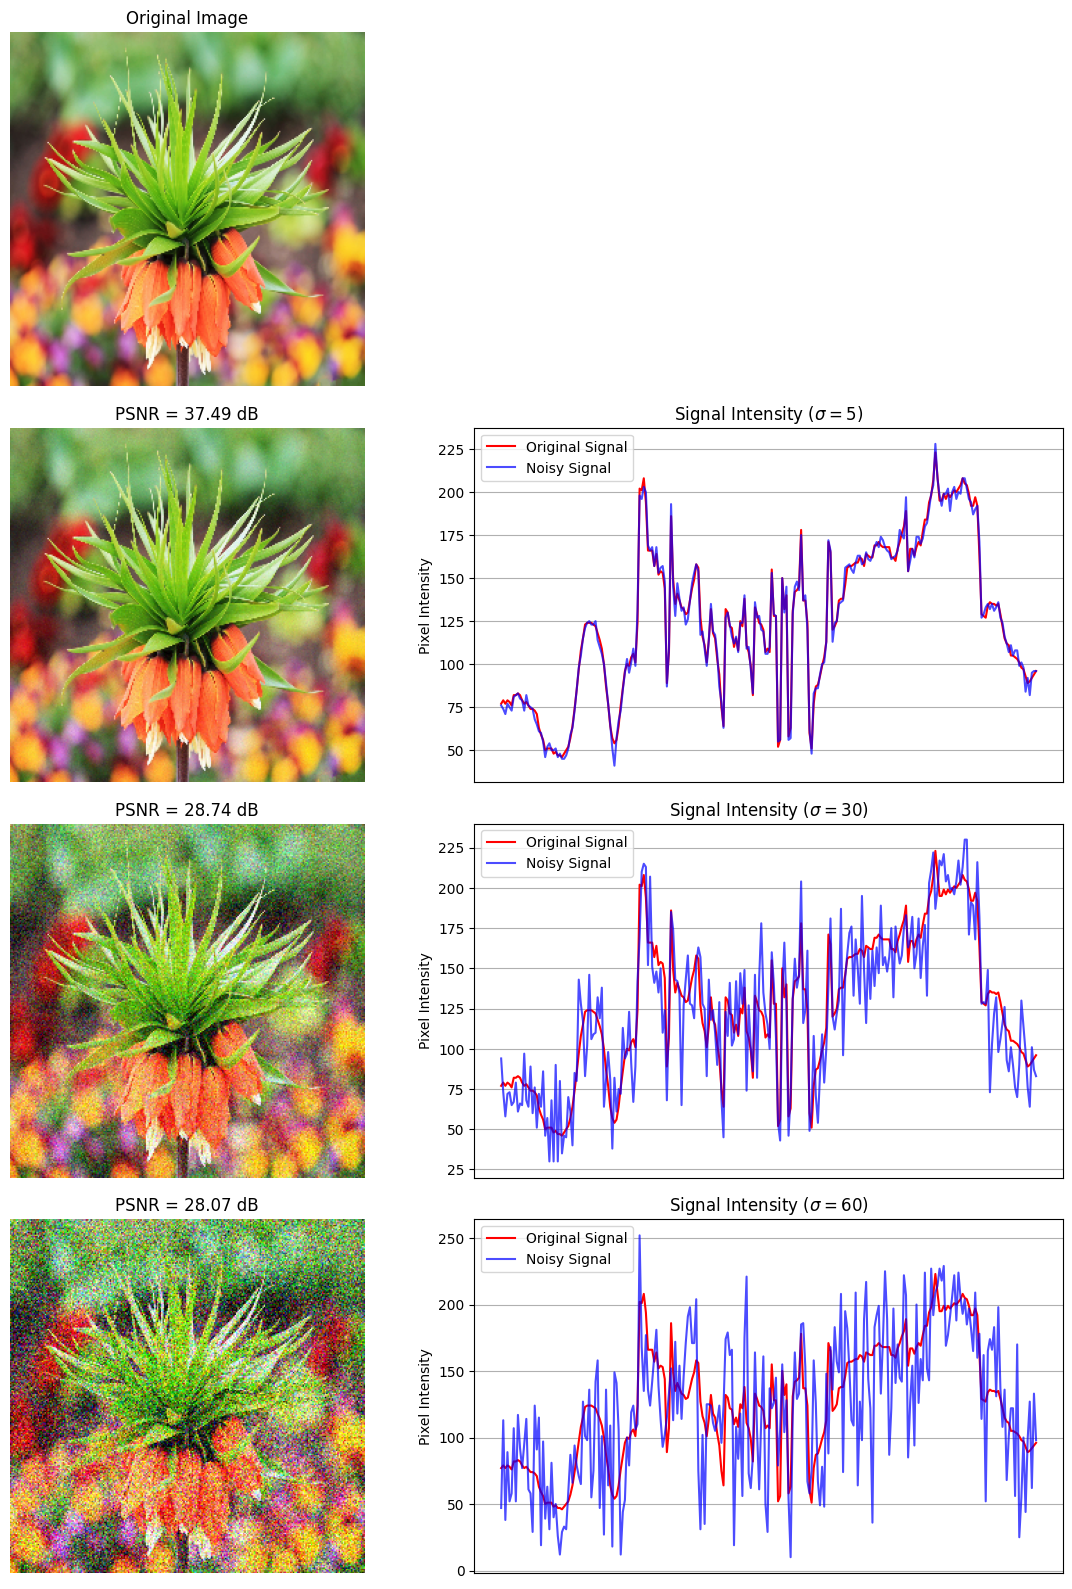
\includegraphics[width=0.6\textwidth]{figures/PSNR_plot.png}
    % \caption{Caption}
    \label{PSNR plot}
\end{figure*}


\textbf{Figure 7.1 Image with different PSNR.} Demonstrates noisy images with their corresponding PSNR values compared to the
original ones. \textbf{Left:} Original image and its noisy version. 
\textbf{Right:} Illustration of how strong noise signals have been added to the original image.
The color image is from the popular \href{https://data.vision.ee.ethz.ch/cvl/DIV2K/}{DIV2K} dataset.
\vspace{-12pt} 

\orangebox{Did you know that...}
{PSNR is not just for images; it can be applied to \textbf{video, audio, or even signal processing}. Anytime we want to
measure the quality of \textbf{reconstructed} signal compared to the \textbf{original}, PSNR could be considered.}

\vspace{-5pt} 

\textbf{Other related metrics}

\vspace{-5pt} 

Modern computer vision problems often focus on generating likely realistic images that are perceptually pleasing to humans,
rather than strictly matching the
target image pixel by pixel. Therefore, PSNR is typically used in conjunction with other modern metrics like Fréchet Inception
Distance (FID) or Inception Score (IS).


